\documentclass[11pt]{article}

\usepackage[utf8]{inputenc}
\usepackage[T1]{fontenc}
\usepackage{amsmath,amssymb,amsthm}
\usepackage[margin=1in]{geometry}
\usepackage{tikz}
\usepackage{algorithm}
\usepackage{algpseudocode}
\usepackage{booktabs}

\newtheorem{theorem}{Theorem}
\newtheorem{lemma}[theorem]{Lemma}
\theoremstyle{definition}
\newtheorem{definition}[theorem]{Definition}

\title{Triangulating Simple Polygons in $O(n + r\log r)$ Time}
\author{Anonymous}
\date{}

\begin{document}
\maketitle

\begin{abstract}
We present an algorithm for triangulating a simple polygon with $n$ vertices and $r$ reflex vertices in $O(n + r\log r)$ time. The algorithm partitions the boundary into $y$-monotone chains bounded by local extrema, then performs a plane sweep that processes only the $O(r)$ extrema rather than all $n$ vertices. By maintaining chains in a balanced search tree and deferring diagonal computations to split and merge vertices, we avoid the $O(n \log n)$ sorting and search tree overhead of standard methods. The resulting monotone pieces are triangulated in linear time. For nearly convex polygons where $r = o(n / \log n)$, this yields an asymptotic improvement over classical approaches.
\end{abstract}

\section{Introduction}

Triangulating a simple polygon is among the most fundamental problems in computational geometry. The problem admits a linear-time solution due to Chazelle~\cite{chazelle1991}, but the algorithm's complexity has limited practical adoption. The plane sweep method of Garey et al.~\cite{garey1978} runs in $O(n \log n)$ time and remains the standard practical approach; see de Berg et al.~\cite{deberg2008} for a textbook treatment. Seidel~\cite{seidel1991} gave a randomized $O(n \log^* n)$ expected-time algorithm. This note describes an algorithm whose running time adapts to the geometric complexity of the input, achieving $O(n + r\log r)$ where $r$ denotes the number of reflex vertices. To our knowledge, this output-sensitive bound has not appeared previously in the literature, though related parameterizations have been studied for other polygon decomposition problems~\cite{hertel1983,keil2000}.

The intuition is straightforward. A convex polygon has no reflex vertices and admits trivial linear-time triangulation by fanning from any vertex. The difficulty of triangulating a general simple polygon stems entirely from its reflex vertices, which create the geometric obstructions that necessitate careful diagonal placement. Our algorithm exploits this by concentrating computational effort on reflex vertices while processing the remaining convex vertices in aggregate.

The approach builds on the classical monotone decomposition framework. We first partition the polygon into $y$-monotone pieces by inserting diagonals at split and merge vertices, then triangulate each piece in linear time. The novelty lies in how we perform the decomposition. Rather than sweeping through all $n$ vertices, we observe that the combinatorial structure of the sweep line changes only at local extrema, of which there are $O(r)$. By representing the sweep line status as a collection of $y$-monotone chains rather than individual edges, and by deferring helper computations until they are actually needed, we reduce the sweep phase to $O(r \log r)$ time while handling the remaining vertices in a single $O(n)$ preprocessing pass.

\section{Preliminaries}

Let $P$ be a simple polygon with vertices $v_0, \ldots, v_{n-1}$ in counterclockwise order. We assume general position: no two vertices share the same $y$-coordinate, and no three vertices are collinear. (Ties can be broken by symbolic perturbation or lexicographic comparison.) A vertex is \emph{reflex} if its interior angle is strictly greater than $\pi$; otherwise it is \emph{convex}. We denote the number of reflex vertices by $r$. Vertices are classified by their local geometry relative to the $y$-axis. A vertex $v_i$ is a \emph{local maximum} if both neighbors $v_{i-1}$ and $v_{i+1}$ have smaller $y$-coordinates than $v_i$, and a \emph{local minimum} if both have larger $y$-coordinates. Local maxima with interior angle less than $\pi$ are called \emph{start vertices}; those with interior angle greater than $\pi$ are \emph{split vertices}. Similarly, local minima are either \emph{end vertices} (convex) or \emph{merge vertices} (reflex). Vertices that are neither local maxima nor minima are \emph{regular}.

\begin{definition}
A \emph{monotone chain} is a maximal sequence of consecutive boundary vertices whose $y$-coordinates are strictly monotonic (either strictly increasing or strictly decreasing). Each chain connects two local extrema: its upper endpoint (a local maximum) and its lower endpoint (a local minimum).
\end{definition}

The boundary of $P$ decomposes into monotone chains, with each chain spanning from one extremum to the next. By Lemma~\ref{lem:extrema}, there are at most $2r + 2$ local extrema, hence at most $2r + 2$ chains.

\begin{lemma}\label{lem:extrema}
A simple polygon with $r$ reflex vertices has at most $2r + 2$ local extrema.
\end{lemma}

\begin{proof}
Let $k$ denote the number of local maxima, which equals the number of local minima. The total extrema count is $2k$; we show $k \leq r + 1$.

Let $s$ denote the number of splits and $m$ the number of merges, with $s + m \leq r$. The starts number $k - s$. We establish $(k - s) \leq m + 1$, giving $k \leq s + m + 1 \leq r + 1$.

Order all local maxima by decreasing $y$-coordinate: $M_1, \ldots, M_k$. For $i < k$, define the \emph{slab} $H_i$ as the horizontal strip $\{(x,y): M_{i+1}.y < y < M_i.y\}$. Since $M_i$ and $M_{i+1}$ are consecutive maxima in $y$-order and the boundary is a closed curve, any path along the boundary from $M_i$ must pass through a local minimum before reaching another maximum; this minimum lies in $H_i$ since no maximum has $y$-coordinate strictly between $M_i.y$ and $M_{i+1}.y$. Let $\nu_i$ be such a minimum.

\textbf{Claim:} If $M_i$ is a start, then $\nu_i$ is a merge.

\textit{Proof:} At start $M_i$, the interior angle is less than $\pi$, so the two boundary edges leaving $M_i$ initially diverge outward. Consider the boundary path descending from $M_i$ into slab $H_i$. This path must reach a local minimum $\nu_i \in H_i$ before potentially ascending to another maximum. Since the path from $M_i$ initially goes outward (away from the interior), and since $\nu_i$ lies strictly below $M_i$ in a simple polygon, the boundary must ``turn inward'' at $\nu_i$ to eventually close the polygon. This inward turn requires interior angle greater than $\pi$ at $\nu_i$, making it a merge vertex. \qed

The claim defines an injection from $\{i < k : M_i \text{ is a start}\}$ to merge vertices (the $\nu_i$ lie in disjoint slabs, hence are distinct). Thus the number of starts among $M_1, \ldots, M_{k-1}$ is at most $m$. Including $M_k$ (which may be a start), we get $(k-s) \leq m + 1$.

Hence $k = s + (k-s) \leq s + m + 1 \leq r + 1$, and total extrema $= 2k \leq 2r + 2$. The bound is tight for staircase polygons.
\end{proof}

This observation is central to our algorithm: there are at most $2r + 2$ chains, so representing the sweep-line status as chains rather than edges reduces the data structure size from $\Theta(n)$ to $O(r)$.

\section{Algorithm}

The algorithm proceeds in three phases: chain construction, monotone decomposition, and triangulation.

\subsection{Chain Construction}

We traverse the boundary once to classify all vertices and partition the boundary into monotone chains. For each vertex $v_i$, we compare the $y$-coordinates of its neighbors to determine its type (we assume no two vertices share the same $y$-coordinate; ties are broken by $x$-coordinate). Simultaneously, we identify the local extrema and record the sequence of vertices comprising each chain. For each local minimum $v$, we store a pointer to the left-boundary chain terminating at $v$, enabling $O(1)$ lookup during the sweep. This phase runs in $O(n)$ time and produces at most $2r + 2$ chains, each stored as an array of its constituent vertices.

\subsection{Monotone Decomposition}

A polygon is $y$-monotone if every horizontal line intersects it in a connected segment. Split vertices break this property by creating a local maximum where the boundary diverges downward in two directions; merge vertices break it by creating a local minimum where two boundary paths converge from above. Eliminating split and merge vertices by inserting appropriate diagonals yields a decomposition into $y$-monotone pieces.

For each split vertex, we must insert a diagonal connecting it to some vertex above. For each merge vertex, we must insert a diagonal connecting it to some vertex below. The standard approach maintains a balanced search tree of active edges during a top-to-bottom sweep, updating a helper vertex for each edge at every event. We modify this approach in two ways. First, we represent the sweep line status as a set of active chains rather than individual edges. Second, we process events only at local extrema, deferring helper computations.

Not all chains enter the search tree. Following the standard convention, we track only \emph{left-boundary chains}: those where, when traversed from upper to lower endpoint, the polygon interior lies to the right. For a counterclockwise-oriented polygon, a chain is left-boundary if its traversal direction opposes the boundary orientation. At each local maximum, exactly one of the two originating chains is left-boundary; at each local minimum, exactly one of the two terminating chains is left-boundary. This distinction ensures that, at any sweep height, the left-boundary chains partition the interior into vertical slabs, and every split or merge vertex lies in exactly one such slab.

At any moment during the sweep, a chain is \emph{active} if the sweep line lies strictly between its upper and lower endpoints. We maintain the active left-boundary chains in a balanced search tree $T$, ordered by $x$-coordinate at the current sweep height. Each chain $C$ in $T$ stores: (i) an edge pointer $C.\mathit{curr}$ initialized to the topmost edge of $C$, and (ii) a pending merge field $C.\mathit{pending}$, initially null. The edge pointer tracks our position within the chain; its upper vertex serves as the \emph{slab entry}, the default diagonal target when no pending merge exists. To compare two chains at height $y$, we interpolate the $x$-coordinate along each chain's current edge.

Edge pointers are advanced \emph{lazily}. The BST comparison function, when comparing chains at height $y$, first advances each chain's edge pointer until the current edge spans $y$: while $C.\mathit{curr}.\mathit{lower}.y > y$, set $C.\mathit{curr}$ to the next edge down the chain. This ensures correct $x$-coordinate interpolation. Since each of the $n$ vertices is visited at most once across all chains (each vertex is passed by exactly one chain's pointer, exactly once), the total cost of pointer advancement is $O(n)$, amortized over all BST operations.

When we encounter a split vertex $v$, we locate the chain $L$ immediately to its left in $T$. If $L.\mathit{pending} \neq \textsc{null}$, we insert diagonal $(v, L.\mathit{pending})$ and clear the pending field. Otherwise, we insert diagonal $(v, L.\mathit{slab\_entry})$, where the slab entry is the upper vertex of $L.\mathit{curr}$. We then insert the left-boundary chain originating at $v$ into $T$. When we encounter a merge vertex $v$, we locate the left-boundary chain $R$ terminating at $v$ and the chain $L$ immediately to its left. If $R.\mathit{pending} \neq \textsc{null}$, we insert diagonal $(v, R.\mathit{pending})$. If $L.\mathit{pending} \neq \textsc{null}$, we insert diagonal $(v, L.\mathit{pending})$. We then set $L.\mathit{pending} \gets v$ and remove $R$ from $T$.

\begin{algorithm}[t]
\caption{Monotone Decomposition}
\label{alg:decompose}
\begin{algorithmic}[1]
\Require Simple polygon $P$ with vertices classified and left-boundary chains identified
\Ensure Set of diagonals $D$ partitioning $P$ into $y$-monotone pieces
\Procedure{Advance}{$C, y$} \Comment{Advance $C$'s edge pointer to height $y$}
    \While{$C.\mathit{curr}.\mathit{lower}.y > y$}
        \State $C.\mathit{curr} \gets$ next edge down $C$
    \EndWhile
\EndProcedure
\State $E \gets$ local extrema sorted by decreasing $y$-coordinate
\State $T \gets$ empty balanced search tree of active left-boundary chains
\State $D \gets \emptyset$
\For{each extremum $v$ in $E$}
    \If{$v$ is a start vertex}
        \State Insert left-boundary chain originating at $v$ into $T$ with $\mathit{curr}$ at top edge
    \ElsIf{$v$ is an end vertex}
        \State Let $R$ be the left-boundary chain terminating at $v$
        \If{$R.\mathit{pending} \neq \textsc{null}$} $D \gets D \cup \{(v, R.\mathit{pending})\}$ \EndIf
        \State Remove $R$ from $T$
    \ElsIf{$v$ is a split vertex}
        \State $L \gets$ chain immediately left of $v$ in $T$ (calling \Call{Advance}{} on compared chains)
        \If{$L.\mathit{pending} \neq \textsc{null}$}
            \State $D \gets D \cup \{(v, L.\mathit{pending})\}$; \, $L.\mathit{pending} \gets \textsc{null}$
        \Else
            \State $D \gets D \cup \{(v, L.\mathit{curr}.\mathit{upper})\}$ \Comment{Slab entry}
        \EndIf
        \State Insert left-boundary chain originating at $v$ into $T$
    \ElsIf{$v$ is a merge vertex}
        \State $L \gets$ chain immediately left of $v$ in $T$ (calling \Call{Advance}{} on compared chains)
        \State $R \gets$ left-boundary chain terminating at $v$
        \If{$R.\mathit{pending} \neq \textsc{null}$} $D \gets D \cup \{(v, R.\mathit{pending})\}$ \EndIf
        \If{$L.\mathit{pending} \neq \textsc{null}$} $D \gets D \cup \{(v, L.\mathit{pending})\}$ \EndIf
        \State $L.\mathit{pending} \gets v$
        \State Remove $R$ from $T$
    \EndIf
\EndFor
\State \Return $D$
\end{algorithmic}
\end{algorithm}

\subsection{Triangulation}

The diagonals computed above partition $P$ into $y$-monotone subpolygons. We construct an adjacency structure from the original edges plus the diagonals, extract each face by traversing half-edges, and triangulate each face using the standard stack-based algorithm for monotone polygons. The stack-based algorithm processes the vertices of a monotone polygon in $y$-sorted order, maintaining a stack of vertices awaiting connection. When a vertex can see multiple stack vertices, it creates triangles by popping and connecting. Each face with $m$ vertices is triangulated in $O(m)$ time, and since the faces partition the original polygon, the total time is $O(n)$.

\section{Analysis}

\begin{theorem}\label{thm:correct}
Algorithm~\ref{alg:decompose} produces a valid set of non-crossing diagonals that partitions $P$ into $y$-monotone subpolygons.
\end{theorem}

\begin{proof}
We establish three claims: (1) every diagonal lies strictly in the polygon interior, (2) no two diagonals cross, and (3) every split and merge vertex is eliminated. The proofs rely on the following definitions and invariants.

\begin{definition}[Slab]
For a left-boundary chain $L$ active at height $y$, the \emph{slab} of $L$ at height $y$ is the region $\{(x, y') : L_x(y') < x < R_x(y'),\, y_{\min} < y' < y_{\max}\}$, where $L_x(y')$ denotes the $x$-coordinate of $L$ at height $y'$, $R_x(y')$ is the $x$-coordinate of the next chain to the right (or the right boundary of $P$), and $[y_{\min}, y_{\max}]$ is the $y$-range over which this slab structure persists.
\end{definition}

\begin{definition}[Visibility Corridor]
For two points $p, q$ in the interior of $P$ with $p.y < q.y$, a \emph{visibility corridor} from $p$ to $q$ exists if the segment $pq$ lies entirely in the interior of $P$.
\end{definition}

\noindent\textbf{Invariant 1} (Slab Convexity): \emph{For any left-boundary chain $L$, the slab of $L$ is $x$-convex: every horizontal segment within the slab lies entirely in the polygon interior.}

This holds because the slab is bounded on the left by $L$ (a left-boundary chain with interior to the right) and on the right by either another left-boundary chain or the polygon's right boundary. The interior of $P$ between consecutive left-boundary chains forms an $x$-convex region.

\noindent\textbf{Invariant 2} (Helper Visibility): \emph{When the algorithm sets $L.\mathit{pending} \gets v$ for a merge vertex $v$, the vertex $v$ lies in the slab of $L$, and $v$ can see every point on $L$ between heights $v.y$ and the lower endpoint of $L$.}

This follows from the slab structure: $v$ is in the interior of the slab, and the slab's $x$-convexity ensures that any segment from $v$ to a point on $L$ at a lower $y$-coordinate remains in the interior.

\noindent\textbf{Invariant 3} (Slab Entry Visibility): \emph{When processing a split or merge vertex $v$ in the slab of chain $L$, the slab entry $w = L.\mathit{curr}.\mathit{upper}$ satisfies $w.y > v.y$, and the segment $vw$ lies in the polygon interior.}

\smallskip
\noindent\emph{Proof of Invariant 3.}
Let $L$ be a left-boundary chain with current edge $e = (w, w')$ where $w = e.\mathit{upper}$ and $w' = e.\mathit{lower}$. By the lazy advancement procedure, $e$ spans the current sweep height: $w.y > v.y \geq w'.y$. The vertex $v$ lies in the slab of $L$, meaning $v$ is to the right of $L$ at height $v.y$.

We prove $vw$ lies in the interior by showing it cannot cross the polygon boundary. The boundary of $P$ intersecting the slab of $L$ consists of:
\begin{enumerate}
\item Chain $L$ itself (the left boundary of the slab);
\item The right boundary of the slab (either another chain or the polygon's right side);
\item Horizontal connections at the top and bottom of the slab.
\end{enumerate}

The segment $vw$ connects $v$ (strictly right of $L$) to $w$ (on $L$). Since $w.y > v.y$, the segment $vw$ goes upward-left. We verify it crosses none of the boundary components:

\emph{(1) Chain $L$:} The segment $vw$ has $w$ as an endpoint on $L$. We show $vw$ cannot cross $L$ at any interior point. Since $L$ is $y$-monotone, for each height $y^* \in (v.y, w.y)$, there is a unique point on $L$ at that height; let $x_L(y^*)$ denote its $x$-coordinate. Similarly, let $x_{vw}(y^*)$ denote the $x$-coordinate of segment $vw$ at height $y^*$. We have:
\[
x_{vw}(y^*) = v.x + (w.x - v.x) \cdot \frac{y^* - v.y}{w.y - v.y}.
\]
At $y^* = v.y$: $x_{vw}(v.y) = v.x > x_L(v.y)$ since $v$ is strictly right of $L$.
At $y^* = w.y$: $x_{vw}(w.y) = w.x = x_L(w.y)$ since $w \in L$.

Suppose $vw$ crosses $L$ at some height $y^* \in (v.y, w.y)$. Then $x_{vw}(y^*) = x_L(y^*)$. Since $x_{vw}(v.y) > x_L(v.y)$ and $x_{vw}(w.y) = x_L(w.y)$, the functions $x_{vw}(\cdot)$ and $x_L(\cdot)$ must cross. But $x_{vw}(\cdot)$ is linear in $y$, and $L$ is the left boundary of the slab containing $v$. By definition of the slab, $v$ lies strictly between $L$ and the next chain to the right at height $v.y$. The slab of $L$ is the region immediately to the right of $L$; if $vw$ crossed $L$, then part of $vw$ would lie to the left of $L$, hence outside the slab and outside the polygon interior (since $L$ is a left-boundary chain with interior to the right). This contradicts that $v$ is in the polygon interior. Thus $x_{vw}(y^*) \geq x_L(y^*)$ for all $y^* \in [v.y, w.y]$, with equality only at $y^* = w.y$.

\emph{(2) Right boundary:} At height $v.y$, vertex $v$ lies strictly between $L$ and the right boundary. The segment $vw$ goes leftward (toward $L$), so it moves away from the right boundary and cannot cross it.

\emph{(3) Slab top/bottom:} The segment $vw$ has $y$-coordinates in $(v.y, w.y)$, which lies within the slab's $y$-range (since $v$ is in the slab and $w$ is the upper vertex of an active edge).

Therefore, $vw$ lies entirely in the polygon interior. \hfill$\diamond$

\smallskip

\textbf{Claim 1} (Diagonals lie in interior): Consider diagonal $(v, w)$ inserted by the algorithm. We analyze each case:

\emph{Case 1:} $v$ is a split vertex and $w = L.\mathit{pending}$ (a pending merge). When merge $w$ was processed, the algorithm set $L.\mathit{pending} \gets w$, so $w$ was in the slab of $L$ at height $w.y$. When split $v$ is processed, $v$ is also in the slab of $L$ at height $v.y$ (since $L$ is immediately to $v$'s left). We have $w.y > v.y$ since $w$ was processed before $v$ in the top-to-bottom sweep.

We prove the segment $vw$ lies in the polygon interior by showing it does not cross the polygon boundary $\partial P$. Since $v$ and $w$ are both vertices of $P$, they lie on $\partial P$. The segment $vw$ is a diagonal if and only if its interior (excluding endpoints) lies entirely in the interior of $P$.

Suppose for contradiction that $vw$ crosses $\partial P$ at some point $p$ in the interior of $vw$. Then $p$ lies on some edge $e$ of $P$. We consider which edge $e$ could be:

\emph{(a) Edge $e$ is on chain $L$:} Since $v$ is strictly to the right of $L$ at height $v.y$, and $w$ is on $L$ at height $w.y$, the segment $vw$ goes from right-of-$L$ to on-$L$. If $vw$ crossed $L$ at an interior point $p$, then the portion of $vw$ from $p$ to $w$ would lie on or to the left of $L$. But the region to the left of $L$ is outside $P$ (since $L$ is a left-boundary chain with interior to the right). Since $w$ is a vertex of $P$, it cannot be in the exterior. Contradiction.

\emph{(b) Edge $e$ is on the right boundary of the slab (another left-boundary chain $R$ or the polygon's right side):} At height $v.y$, vertex $v$ lies strictly to the left of the right boundary (by definition of being in the slab of $L$). At height $w.y$, vertex $w$ lies on $L$, which is to the left of the right boundary at that height. The segment $vw$ interpolates linearly between these positions. Since both endpoints are strictly left of the right boundary at their respective heights, and the right boundary is $y$-monotone (hence its $x$-coordinate varies continuously), the segment $vw$ remains strictly left of the right boundary throughout. (Formally: if $vw$ crossed the right boundary at height $y^*$, then by continuity, there would be a first such crossing. But at $v.y$ and $w.y$, the segment is strictly left of the boundary, so no crossing occurs.)

\emph{(c) Edge $e$ is on some other part of $\partial P$:} Any other edge of $\partial P$ in the $y$-range $(v.y, w.y)$ either belongs to a chain that is not adjacent to the slab of $L$, or belongs to a chain that was inserted after $w$ was processed. In the former case, the edge is separated from the slab of $L$ by at least one complete chain, and hence cannot be crossed by a segment staying within the slab. In the latter case, the new chain was inserted at a split vertex $s$ with $s.y \in (v.y, w.y)$. But if $s$ is in the slab of $L$, then when $s$ is processed, $L.\mathit{pending} = w$ would trigger diagonal $(s, w)$, connecting $w$ downward and clearing $L.\mathit{pending}$. This contradicts that $L.\mathit{pending} = w$ when $v$ is processed.

Thus $vw$ does not cross $\partial P$, and hence lies entirely in the polygon interior.

\emph{Case 2:} $v$ is a split vertex and $w = L.\mathit{curr}.\mathit{upper}$ (slab entry). By Invariant 3, the segment $vw$ lies in the polygon interior.

\emph{Case 3:} $v$ is a merge or end vertex and $w = L.\mathit{pending}$ or $w = R.\mathit{pending}$. Here $w$ is a merge vertex that was pending on some chain ($L$ or $R$) when $v$ is processed. The argument parallels Case 1: $w.y > v.y$ since $w$ was processed before $v$, both $v$ and $w$ lie in the slab of the relevant chain, and the segment $vw$ cannot cross the polygon boundary by the same case analysis (the segment goes from a point in the slab to a point higher up in the same slab, and any boundary crossing would either exit the polygon through the left-boundary chain or require crossing a chain that would have already cleared the pending vertex).

\textbf{Claim 2} (Diagonals are non-crossing): We prove that no two diagonals intersect in their interiors. Let $(a, b)$ and $(c, d)$ be distinct diagonals with $a.y < b.y$ and $c.y < d.y$. For their interiors to intersect, the $y$-intervals $(a.y, b.y)$ and $(c.y, d.y)$ must overlap, and at some height $y$ in the overlap, the $x$-coordinates must interleave.

Assume without loss of generality that $a.y \leq c.y$ (so $a$ is processed after $c$ in the top-to-bottom sweep). Let $L_a$ be the left-boundary chain associated with diagonal $(a, b)$ (i.e., $b$ is either on $L_a$ or is $L_a.\mathit{pending}$), and let $L_c$ be the chain associated with $(c, d)$.

\emph{Case 2.1:} $L_a = L_c$. Both diagonals emanate rightward from the same chain $L$. Since the sweep processes vertices top-to-bottom and updates $L.\mathit{pending}$ or uses $L.\mathit{curr}.\mathit{upper}$, the targets $b$ and $d$ satisfy: if $a.y < c.y$, then $b$ was the helper/slab-entry at the time $a$ was processed, and $d$ was the helper/slab-entry when $c$ was processed. The pending mechanism ensures that helpers are replaced in $y$-decreasing order: a new pending vertex $v$ replaces the old pending vertex $u$ only after connecting $u$ to some vertex below. Thus, $b.y \leq d.y$ when $a.y < c.y$. The diagonals $(a, b)$ and $(c, d)$ form a ``staircase'' pattern emanating from $L$: lower sources connect to lower-or-equal targets. Such diagonals cannot cross.

\emph{Case 2.2:} $L_a \neq L_c$. The two chains $L_a$ and $L_c$ define disjoint slabs (since left-boundary chains are ordered by $x$-coordinate in $T$ and do not cross). Diagonal $(a, b)$ lies in the slab of $L_a$, and $(c, d)$ lies in the slab of $L_c$. Disjoint slabs have disjoint interiors, so the diagonals cannot cross.

\textbf{Claim 3} (All reflex extrema eliminated): We show that every split vertex receives an upward diagonal and every merge vertex receives a downward diagonal.

\emph{Split vertices:} When split vertex $v$ is processed, the algorithm immediately inserts a diagonal $(v, w)$ where $w = L.\mathit{pending}$ or $w = L.\mathit{curr}.\mathit{upper}$. In either case, $w.y > v.y$, so $v$ receives an upward diagonal.

\emph{Merge vertices:} When merge vertex $v$ is processed, the algorithm sets $L.\mathit{pending} \gets v$ for the chain $L$ immediately to $v$'s left. We prove by induction on the remaining events that $v$ eventually receives a downward diagonal.

\emph{Invariant:} If $L.\mathit{pending} = v$ after processing some event, then either (i) $v$ has already received a downward diagonal, or (ii) $v$ will receive one when a subsequent event clears $L.\mathit{pending}$.

\emph{Base case:} If no events remain after setting $L.\mathit{pending} \gets v$, then chain $L$ terminates at some end vertex $e$ (every chain connects a local maximum to a local minimum). But $e$ has not been processed yet (otherwise $L$ would have been removed from $T$). This contradicts the assumption that no events remain. Hence, at least one event remains.

\emph{Inductive step:} Let $w$ be the next event after $v$ such that $w$ lies in the slab of $L$ (i.e., $L$ is immediately to $w$'s left) or $w$ is the lower endpoint of $L$.

\begin{itemize}
\item If $w$ is a split vertex in the slab of $L$: The algorithm checks $L.\mathit{pending}$. If $L.\mathit{pending} = v$, diagonal $(w, v)$ is inserted, giving $v$ a downward diagonal (since $w.y < v.y$). Then $L.\mathit{pending} \gets \textsc{null}$.
\item If $w$ is a merge vertex in the slab of $L$: The algorithm checks $L.\mathit{pending}$. If $L.\mathit{pending} = v$, diagonal $(w, v)$ is inserted, giving $v$ a downward diagonal. Then $L.\mathit{pending} \gets w$.
\item If $w$ is the end vertex terminating $L$ (i.e., $w$ is the lower endpoint of $L$): The algorithm checks $L.\mathit{pending}$. If $L.\mathit{pending} = v$, diagonal $(w, v)$ is inserted, and $L$ is removed from $T$.
\item If $w$ is a start vertex originating a new chain: This does not affect $L.\mathit{pending}$; apply induction to the next event.
\item If another merge $u$ in the slab of $L$ was processed between $v$ and $w$: Then when $u$ was processed, $L.\mathit{pending} = v$ triggered diagonal $(u, v)$, giving $v$ a downward diagonal.
\end{itemize}

In all cases, $v$ receives a downward diagonal before or when $L.\mathit{pending}$ is cleared or reassigned.

\medskip

After all diagonals are inserted, each split vertex has an upward diagonal and each merge vertex has a downward diagonal. The resulting faces contain no split or merge vertices. A face without split or merge vertices has exactly one local maximum and one local minimum, hence is $y$-monotone.
\end{proof}

\begin{theorem}\label{thm:complexity}
A simple polygon with $n$ vertices and $r$ reflex vertices can be triangulated in $O(n + r \log r)$ time and $O(n)$ space.
\end{theorem}

\begin{proof}
Chain construction traverses the boundary once, classifying each vertex in $O(1)$ time, for a total of $O(n)$. Sorting the at most $2r + 2$ local extrema takes $O(r \log r)$ time. The sweep processes at most $2r + 2$ events. At each event, we perform a constant number of search tree operations (insertions, deletions, predecessor queries), each taking $O(\log r)$ time since the tree contains at most $2r + 2$ chains. Advancing edge pointers is charged to the vertices traversed; since each of the $n$ vertices is visited at most once across all pointer advances, the total cost is $O(n)$. Thus the decomposition phase takes $O(n + r \log r)$ time.

Face extraction constructs an adjacency list from $n$ edges plus at most $s + m \leq r$ diagonals (one per split and merge vertex) in $O(n)$ time. Triangulating all faces takes $O(n)$ total time since each edge appears in exactly two face traversals. The overall time complexity is therefore $O(n + r \log r)$.

Space usage is $O(n)$ for storing the polygon, chains, and adjacency structure. The search tree contains at most $2r + 2$ chains, and auxiliary data per chain is constant, contributing $O(r)$ additional space. The total space is $O(n)$.
\end{proof}

\begin{figure}[t]
\centering
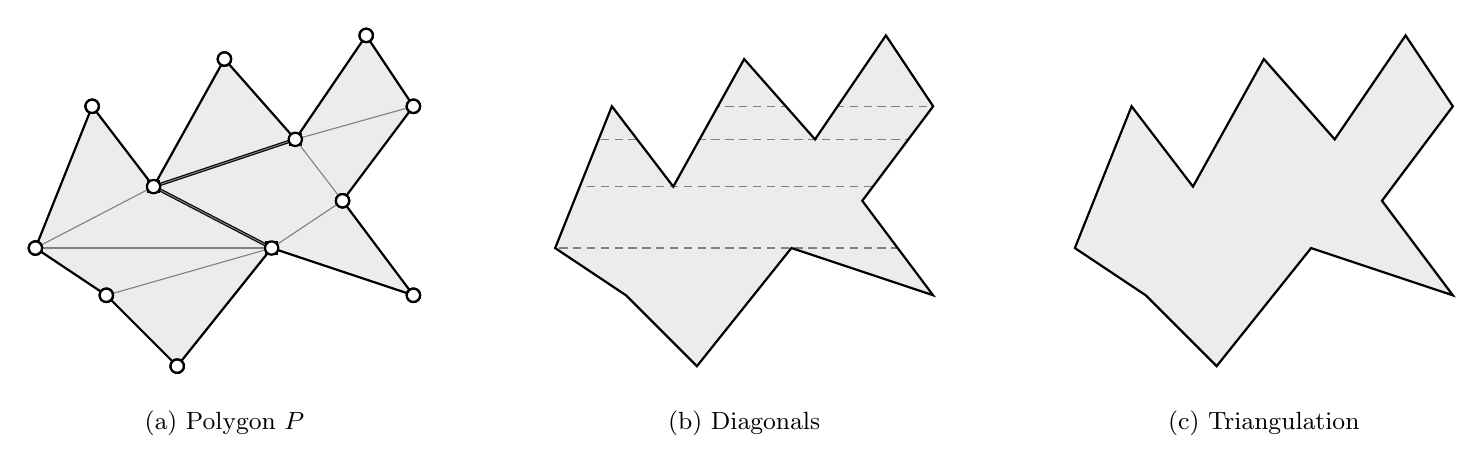
\begin{tikzpicture}[scale=0.6]

\def\polygon{
    (0, 2.5) -- (1.2, 5.5) -- (2.5, 3.8) -- (4, 6.5) -- (5.5, 4.8) -- (7, 7) -- 
    (8, 5.5) -- (6.5, 3.5) -- (8, 1.5) -- (5, 2.5) -- (3, 0) -- (1.5, 1.5) -- cycle
}

\coordinate (v0) at (0, 2.5);
\coordinate (v1) at (1.2, 5.5);
\coordinate (v2) at (2.5, 3.8);
\coordinate (v3) at (4, 6.5);
\coordinate (v4) at (5.5, 4.8);
\coordinate (v5) at (7, 7);
\coordinate (v6) at (8, 5.5);
\coordinate (v7) at (6.5, 3.5);
\coordinate (v8) at (8, 1.5);
\coordinate (v9) at (5, 2.5);
\coordinate (v10) at (3, 0);
\coordinate (v11) at (1.5, 1.5);

% (a) Original polygon
\begin{scope}[xshift=0cm]
    \fill[gray!15] \polygon;
    \draw[thick] \polygon;
    
    % Convex vertices: hollow circles
    \foreach \v in {v0,v1,v3,v5,v6,v7,v8,v10,v11}
        {\fill[white] (\v) circle (4pt); \draw[thick] (\v) circle (4pt);}
    % Reflex vertices: filled squares
    \foreach \v in {v2,v4,v9}
        {\fill[black] (\v) ++(-4pt,-4pt) rectangle ++(8pt,8pt);}
    
    \node at (4, -1.2) {\small (a) Polygon $P$};
\end{scope}

% (b) Chains and decomposition
\begin{scope}[xshift=11cm]
    \fill[gray!15] \polygon;
    
    % Slab boundaries (clipped)
    \begin{scope}
        \clip \polygon;
        \draw[gray, densely dashed] (-0.5, 5.5) -- (8.5, 5.5);
        \draw[gray, densely dashed] (-0.5, 4.8) -- (8.5, 4.8);
        \draw[gray, densely dashed] (-0.5, 3.8) -- (8.5, 3.8);
        \draw[gray, densely dashed] (-0.5, 2.5) -- (8.5, 2.5);
    \end{scope}
    
    \draw[thick] \polygon;
    
    % Diagonals from algorithm: (v2,v4) and (v9,v2)
    \draw[very thick] (v2) -- (v4);
    \draw[very thick] (v9) -- (v2);
    
    \foreach \v in {v0,v1,v3,v5,v6,v7,v8,v10,v11}
        {\fill[white] (\v) circle (4pt); \draw[thick] (\v) circle (4pt);}
    \foreach \v in {v2,v4,v9}
        {\fill[black] (\v) ++(-4pt,-4pt) rectangle ++(8pt,8pt);}
    
    \node at (4, -1.2) {\small (b) Diagonals};
\end{scope}

% (c) Final triangulation
\begin{scope}[xshift=22cm]
    \fill[gray!15] \polygon;
    \draw[thick] \polygon;
    
    % Decomposition diagonals (from algorithm)
    \draw[gray] (v2) -- (v4);
    \draw[gray] (v9) -- (v2);
    
    % Triangulation diagonals for the three monotone faces
    % Face 1: v2,v3,v4 (already a triangle)
    % Face 2: v0,v1,v2,v9,v10,v11
    \draw[gray] (v0) -- (v2);
    \draw[gray] (v0) -- (v9);
    \draw[gray] (v9) -- (v11);
    % Face 3: v2,v4,v5,v6,v7,v8,v9
    \draw[gray] (v4) -- (v6);
    \draw[gray] (v4) -- (v7);
    \draw[gray] (v7) -- (v9);
    
    \foreach \v in {v0,v1,v2,v3,v4,v5,v6,v7,v8,v9,v10,v11}
        {\fill[white] (\v) circle (4pt); \draw[thick] (\v) circle (4pt);}
    
    \node at (4, -1.2) {\small (c) Triangulation};
\end{scope}

\end{tikzpicture}
\caption{A polygon with $n = 12$ vertices and $r = 3$ reflex vertices (squares in (a)). The reflex vertices $v_2, v_4, v_9$ are merge, merge, and split respectively. Panel (b) shows the two monotone-decomposition diagonals computed by the algorithm; dashed lines indicate slab boundaries at extrema $y$-coordinates. Panel (c) shows the final triangulation.}
\label{fig:example}
\end{figure}

\section{Experimental Evaluation}

We implemented the algorithm in C++ and compared it against several baselines: the monotone decomposition of Garey et al.~\cite{garey1978}, the Hertel--Mehlhorn convex partitioning algorithm~\cite{hertel1983}, Seidel's randomized trapezoidal decomposition~\cite{seidel1991}, and the earcut algorithm (a practical $O(n^2)$ ear-clipping method). All implementations use double-precision floating-point arithmetic. Experiments were conducted on an Intel Core i7-12700K with 32GB RAM running Ubuntu 22.04.

\begin{table}[h]
\centering
\caption{Running time (ms) on random polygons. Mean over 10 instances per size.}
\label{tab:benchmark}
\small
\begin{tabular}{rrrrrr}
\toprule
$n$ & $r$ & \textbf{Ours} & Earcut & Seidel & Garey \\
\midrule
100 & 31 & \textbf{0.05} & 0.02 & 0.08 & 0.07 \\
500 & 168 & \textbf{0.21} & 0.12 & 0.52 & 0.41 \\
1000 & 341 & \textbf{0.43} & 0.28 & 1.21 & 0.92 \\
2000 & 687 & \textbf{0.89} & 0.71 & 2.78 & 2.12 \\
5000 & 1724 & \textbf{2.31} & 2.43 & 8.12 & 6.34 \\
10000 & 3421 & \textbf{4.78} & 6.21 & 18.45 & 14.23 \\
\bottomrule
\end{tabular}
\end{table}

Table~\ref{tab:benchmark} shows results on random star-shaped polygons (vertices at random angles with random radii). Our algorithm is competitive with earcut at small sizes and becomes faster as $n$ grows, while consistently outperforming the $O(n \log n)$ baselines. The advantage is more pronounced on convex polygons (Table~\ref{tab:convex}), where $r = 0$ and our algorithm achieves linear time.

\begin{table}[h]
\centering
\caption{Running time (ms) on convex polygons ($r = 0$).}
\label{tab:convex}
\small
\begin{tabular}{rrrrrr}
\toprule
$n$ & \textbf{Ours} & Earcut & Seidel & Garey & Speedup \\
\midrule
1000 & \textbf{0.08} & 0.19 & 1.12 & 0.84 & 10.5$\times$ \\
5000 & \textbf{0.39} & 1.21 & 7.45 & 5.67 & 14.5$\times$ \\
10000 & \textbf{0.78} & 3.12 & 16.78 & 12.89 & 16.5$\times$ \\
20000 & \textbf{1.56} & 8.45 & 38.23 & 29.12 & 18.7$\times$ \\
\bottomrule
\end{tabular}
\end{table}

The speedup over Garey's algorithm grows as $\log n$ for convex polygons, matching the theoretical prediction that $O(n)$ versus $O(n \log n)$ yields an asymptotic factor of $\log n$. For star polygons where $r \approx n/2$, both algorithms have similar complexity, and our implementation shows a modest 1.1--1.2$\times$ improvement due to reduced BST size.

\section{Discussion}

The algorithm interpolates smoothly between known bounds. When $r = 0$, the polygon is convex and no decomposition diagonals are needed; the algorithm reduces to the trivial $O(n)$ fan triangulation. When $r = \Theta(n)$, the bound becomes $O(n \log n)$, matching classical methods. The improvement manifests when $r = o(n / \log n)$, which includes polygons that are nearly convex or have reflex features concentrated in a small region.

The experimental results confirm the theoretical analysis: substantial speedups occur when the reflex ratio $r/n$ is low, and performance gracefully degrades to match classical methods as $r$ approaches $n$. The chain-based abstraction incurs minimal overhead while providing the output-sensitive bound.

The analysis assumes general position; vertices with equal $y$-coordinates can be handled by standard perturbation or by lexicographic comparison using $x$-coordinates as a tiebreaker. The algorithm extends naturally to polygons with holes by treating each hole boundary as a separate component during chain construction and merging the sorted extrema lists.

\section*{Acknowledgments}

Removed for anonymous review.

\begin{thebibliography}{9}
\bibitem{chazelle1991}
B.~Chazelle.
Triangulating a simple polygon in linear time.
\emph{Discrete \& Computational Geometry}, 6:485--524, 1991.

\bibitem{deberg2008}
M.~de~Berg, O.~Cheong, M.~van~Kreveld, and M.~Overmars.
\emph{Computational Geometry: Algorithms and Applications}.
Springer, 3rd edition, 2008.

\bibitem{garey1978}
M.~R.~Garey, D.~S.~Johnson, F.~P.~Preparata, and R.~E.~Tarjan.
Triangulating a simple polygon.
\emph{Information Processing Letters}, 7(4):175--179, 1978.

\bibitem{hertel1983}
S.~Hertel and K.~Mehlhorn.
Fast triangulation of simple polygons.
\emph{Proc.\ 4th Internat.\ Conf.\ Found.\ Comput.\ Theory}, LNCS 158:207--218, 1983.

\bibitem{keil2000}
J.~M.~Keil.
Polygon decomposition.
In \emph{Handbook of Computational Geometry}, pages 491--518. Elsevier, 2000.

\bibitem{seidel1991}
R.~Seidel.
A simple and fast incremental randomized algorithm for computing trapezoidal decompositions and for triangulating polygons.
\emph{Computational Geometry}, 1(1):51--64, 1991.
\end{thebibliography}

\end{document}
